\textit{Response.} 

We begin by solving the complex OU equation. In particular, we utilize the integration factor $e^{-\gpr{-a + i\,\omega}\,t}$:

\begin{alignat}{2}
	& & \dv{x}{t} &= \gpr{-a + i\,\omega}\,x + f + \sigma\,\func{\dot{W}}{t} \nonumber \\
	\impl & & e^{-\gpr{-a + i\,\omega}\,t}\,\dv{x}{t} - \gpr{-a + i\,\omega}\,e^{-\gpr{-a + i\,\omega}\,t}\,x &= e^{-\gpr{-a + i\,\omega}\,t}\,f + \sigma\,e^{-\gpr{-a + i\,\omega}\,t}\,\func{\dot{W}}{t} \nonumber \\
	\impl & & \dv{t}\gbkt{e^{-\gpr{-a + i\,\omega}\,t}\,x} &= e^{-\gpr{-a + i\,\omega}\,t}\,f + \sigma\,e^{-\gpr{-a + i\,\omega}\,t}\,\func{\dot{W}}{t} \nonumber \\
	\impl & & e^{-\gpr{-a + i\,\omega}\,t}\,\func{x}{t} - \func{x}{0} &= \int_{0}^{t} e^{-\gpr{-a + i\,\omega}\,s}\,\func{f}{s}\,ds + \sigma\,\int_{0}^{t} e^{-\gpr{-a + i\,\omega}\,s}\,d\func{W}{s} \nonumber \\
	\impl & & \func{x}{t} &= e^{\gpr{-a + i\,\omega}\,t}\,\func{x}{0} + \int_{0}^{t} e^{\gpr{-a + i\,\omega}\,\gpr{t - s}}\,\func{f}{s}\,ds \nonumber \\
	& & &\qquad + \sigma\,\int_{0}^{t} e^{\gpr{-a + i\,\omega}\,\gpr{t - s}}\,d\func{W}{s}.
\end{alignat}

To obtain the expected value $\func{x}{t}$, we must calculate the expected value of each term on the right-hand side. The first term contains only one random part, being $\func{x}{0}$, and so its expected value is straightforward. The second term is entirely determinisitc, and therefore is equal to its expected value. To calculate the expected value of the third term on the right, we appeal to the second identity given in slide 6 of Lecture 3:

\begin{equation}
	\ev{\sigma\,\int_{0}^{t} e^{\gpr{-a + i\,\omega}\,\gpr{t - s}}\,d\func{W}{s}} = 0.
\end{equation}

Therefore, the time evolution of the expected value of $\func{x}{t}$ is given by

\begin{equation}
	\ev{\func{x}{t}} = e^{\gpr{-a + i\,\omega}\,t}\,\ev{\func{x}{0}} + \int_{0}^{t} e^{\gpr{-a + i\,\omega}\,\gpr{t - s}}\,\func{f}{s}\,ds.
\end{equation}

For a constant deterministic forcing $\func{f}{t} = f$, this simplifies to

\begin{equation}
	\ev{\func{x}{t}} = e^{\gpr{-a + i\,\omega}\,t}\,\ev{\func{x}{0}} + \frac{f}{-a + i\,\omega}\,\gpr{e^{\gpr{-a + i\,\omega}t} - 1}.
\end{equation}

When discussing the variance of a complex variable, it is important to discuss both the variance $\vr{\func{x}{t}}$ and the pseusdo-variance $\pvr{\func{x}{t}}$. They are defined as follows

\begin{subequations}
	\begin{align}
		\vr{\func{x}{t}} &:= \ev{\abs{\func{x}{t} - \ev{\func{x}{t}}}^2}, \\
		\pvr{\func{x}{t}} &:= \ev{\gpr{\func{x}{t} - \ev{\func{x}{t}}}^2}.
	\end{align}
\end{subequations}

Writing $\func{x}{t} = \func{a}{t} + i\,\func{b}{t}$ (with $\func{a}{t}$, $\func{b}{t}$ real), we may find the variances and covariances of $\func{a}{t}$, $\func{b}{t}$ using the variances and pseudo-variance of $\func{x}{t}$

\begin{subequations}
	\begin{align}
		\vr{\func{a}{t}} &= \frac{1}{2}\,\re{\vr{\func{x}{t}} + \pvr{\func{x}{t}}}, \\
		\cov{\func{a}{t}}{\func{b}{t}} &= \frac{1}{2}\,\im{-\vr{\func{x}{t}} + \pvr{\func{x}{t}}}, \\
		\cov{\func{b}{t}}{\func{a}{t}} &= \frac{1}{2}\,\im{\vr{\func{x}{t}} + \pvr{\func{x}{t}}}, \\
		\vr{\func{b}{t}} &= \frac{1}{2}\,\re{\vr{\func{x}{t}} - \pvr{\func{x}{t}}}.
	\end{align}
\end{subequations}

and conversely

\begin{subequations}
	\begin{align}
		\vr{\func{x}{t}} &= \vr{\func{a}{t}} + \vr{\func{b}{t}} - i\,\gpr{\cov{\func{a}{t}}{\func{b}{t}} - \cov{\func{b}{t}}{\func{a}{t}}}, \\
		\pvr{\func{x}{t}} &= \vr{\func{a}{t}} - \vr{\func{b}{t}} + i\,\gpr{\cov{\func{a}{t}}{\func{b}{t}} + \cov{\func{b}{t}}{\func{a}{t}}}.
	\end{align}
\end{subequations}

We begin by calculating the time evolution of the variance of $\func{x}{t}$. The difference $\func{x}{t} - \ev{\func{x}{t}}$ is given by

\begin{equation}
	\func{x}{t} - \ev{\func{x}{t}} = e^{\gpr{-a + i\,\omega}\,t}\,\gpr{\func{x}{0} - \ev{\func{x}{0}}} + \sigma\,\int_{0}^{t} e^{\gpr{-a + i\,\omega}\,\gpr{t - s}}\,d\func{W}{s}.
\end{equation}

The complex norm of this difference contains four terms

\begin{align}
	\abs{\func{x}{t} - \ev{\func{x}{t}}}^2 &= e^{-2\,a\,t}\,\abs{\func{x}{0} - \ev{\func{x}{0}}}^2 \nonumber \\
			&\qquad + \sigma\,e^{\gpr{-a + i\,\omega}\,t}\,\gpr{\func{x}{0} - \ev{\func{x}{0}}}\,\int_{0}^{t} e^{-\gpr{a + i\,\omega}\,\gpr{t - s}}\,\overline{d\func{W}{s}} \nonumber \\
			&\qquad + \sigma\,e^{-\gpr{a + i\,\omega}\,t}\,\overline{\gpr{\func{x}{0} - \ev{\func{x}{0}}}}\,\int_{0}^{t} e^{\gpr{-a + i\,\omega}\,\gpr{t - s}}\,d\func{W}{s} \nonumber \\
			&\qquad + \sigma^2\,\gpr{\int_{0}^{t} e^{\gpr{-a + i\,\omega}\,\gpr{t - s}}\,d\func{W}{s}}\,\gpr{\int_{0}^{t} e^{-\gpr{a + i\,\omega}\,\gpr{t - s}}\,\overline{d\func{W}{s}}}
\end{align}

The expected value of the first term is given by $e^{-2\,a\,t}\,\vr{\func{x}{0}}$. Assuming that $\func{x}{0}$ is independent of the white noise $\func{\dot{W}}{s}$, the expected value of the second and third terms are zero\footnote{\label{fnt:int_against_dW}See the second identity given in slide 6 of Lecture 3.}. The fourth term requires further calculation. Specifically, by decompsing $d\func{W}{s} = \frac{1}{\sqrt{2}}\,\gpr{d\func{U}{s} + i\,d\func{V}{s}}$ into its independent real and imaginary parts, we may utilize the It\^{o} isometry to calculate its expected value. Specifically, the It\^{o} isometry states that for ``nice'' determinstic functions $\func{f}{s}$, $\func{g}{s}$, we have

\begin{equation}
	\ev{\gpr{\int_{0}^{t} \func{f}{s}\,d\func{W}{s}}\,\gpr{\int_{0}^{t} \func{g}{s}\,d\func{W}{s}}} = \int_{0}^{t} \func{f}{s}\,\func{g}{s}\,ds.
\end{equation}

We calculate

\begin{align}
	\text{E}\left[\gpr{\int_{0}^{t} e^{\gpr{-a + i\,\omega}\,\gpr{t - s}}\,d\func{W}{s}}\right.\,&\left.\gpr{\int_{0}^{t} e^{-\gpr{a + i\,\omega}\,\gpr{t - s}}\,\overline{d\func{W}{s}}}\right] \nonumber \\
			&= \frac{1}{2}\,\ev{\gpr{\int_{0}^{t} e^{\gpr{-a + i\,\omega}\,\gpr{t - s}}\,d\func{U}{s}}\,\gpr{\int_{0}^{t} e^{-\gpr{a + i\,\omega}\,\gpr{t - s}}\,d\func{U}{s}}} \nonumber \\
				&\qquad - \frac{1}{2}\,i\,\ev{\gpr{\int_{0}^{t} e^{\gpr{-a + i\,\omega}\,\gpr{t - s}}\,d\func{U}{s}}\,\gpr{\int_{0}^{t} e^{-\gpr{a + i\,\omega}\,\gpr{t - s}}\,d\func{V}{s}}} \nonumber \\
				&\qquad + \frac{1}{2}\,i\,\ev{\gpr{\int_{0}^{t} e^{\gpr{-a + i\,\omega}\,\gpr{t - s}}\,d\func{V}{s}}\,\gpr{\int_{0}^{t} e^{-\gpr{a + i\,\omega}\,\gpr{t - s}}\,d\func{U}{s}}} \nonumber \\
				&\qquad + \frac{1}{2}\,\ev{\gpr{\int_{0}^{t} e^{\gpr{-a + i\,\omega}\,\gpr{t - s}}\,d\func{V}{s}}\,\gpr{\int_{0}^{t} e^{-\gpr{a + i\,\omega}\,\gpr{t - s}}\,d\func{V}{s}}} \nonumber \\
			&= \frac{1}{2}\,\int_{0}^{t} e^{-2\,a\,\gpr{t - s}}\,ds \nonumber \\
				&\qquad - 0 \nonumber \\
				&\qquad + 0 \nonumber \\
				&\qquad + \frac{1}{2}\,\int_{0}^{t} e^{-2\,a\,\gpr{t - s}}\,ds \nonumber \\
			&= \frac{1}{2\,a}\,\gpr{1 - e^{-2\,a\,t}}.
\end{align}

Combining this with the other three terms, we find that

\begin{equation}
	\vr{\func{x}{t}} = e^{-2\,a\,t}\,\vr{\func{x}{0}} + \frac{\sigma^2}{2\,a}\,\gpr{1 - e^{-2\,a\,t}}.
\end{equation}

We now calculate the time evolution of the pseudo-variance of $\func{x}{t}$, we begin by calculating the square of the difference $\func{x}{t} - \ev{\func{x}{t}}$ which yields three terms

\begin{align}
	\gpr{\func{x}{t} - \ev{\func{x}{t}}}^2 &= \gpr{e^{\gpr{-a + i\,\omega}\,t}\,\gpr{\func{x}{0} - \ev{\func{x}{0}}} + \sigma\,\int_{0}^{t} e^{\gpr{-a + i\,\omega}\,\gpr{t - s}}\,d\func{W}{s}}^2 \nonumber \\
		&= \gpr{e^{\gpr{-a + i\,\omega}\,t}\,\gpr{\func{x}{0} - \ev{\func{x}{0}}}}^2 \nonumber \\
			&\qquad + 2\,\sigma\,\gpr{\func{x}{0} - \ev{\func{x}{0}}}\,\int_{0}^{t} e^{\gpr{-a + i\,\omega}\,\gpr{t - s}}\,d\func{W}{s} \nonumber \\
			&\qquad + \sigma^2\,\gpr{\int_{0}^{t} e^{\gpr{-a + i\,\omega}\,\gpr{t - s}}\,d\func{W}{s}}^2
\end{align}

The expected value of the first term on the right-hand side is simply $e^{\gpr{-a + i\,\omega}\,t}\,\pvr{\func{x}{0}}$. Again using the assumption that $\func{x}{0}$ is independent of the white-noise term, we find that the expected value of the second term on the right-hand side is zero\footref{fnt:int_against_dW}. To calculate the expected value of the third term on the right-hand side, we appeal to the It\^{o} isometry. Hence,

\begin{align}
	\ev{\gpr{\int_{0}^{t} e^{\gpr{-a + i\,\omega}\,\gpr{t - s}}\,d\func{W}{s}}^2} &= \frac{1}{2}\,\ev{\gpr{\int_{0}^{t} e^{\gpr{-a + i\,\omega}\,\gpr{t - s}}\,d\func{U}{s}}^2} \nonumber \\
			&\qquad + i\,\ev{\gpr{\int_{0}^{t} e^{\gpr{-a + i\,\omega}\,\gpr{t - s}}\,d\func{U}{s}}\,\gpr{\int_{0}^{t} e^{\gpr{-a + i\,\omega}\,\gpr{t - s}}\,d\func{V}{s}}} \nonumber \\
			&\qquad - \frac{1}{2}\,\ev{\gpr{\int_{0}^{t} e^{\gpr{-a + i\,\omega}\,\gpr{t - s}}\,d\func{V}{s}}^2} \nonumber \\
		&= \frac{1}{2}\,\int_{0}^{t} e^{2\,\gpr{-a + i\,\omega}\,\gpr{t - s}}\,ds \nonumber \\
			&\qquad + 0 \nonumber \\
			&\qquad - \frac{1}{2}\,\int_{0}^{t} e^{2\,\gpr{-a + i\,\omega}\,\gpr{t - s}}\,ds \nonumber \\
		&= 0
\end{align}

Therefore, the time evolution of the pseudo-variance of $\func{x}{t}$ is given by

\begin{equation}
	\pvr{\func{x}{t}} = e^{\gpr{-a + i\,\omega}\,t}\,\pvr{\func{x}{0}}.
\end{equation}

We may combine the variance and pseudo-variances of $\func{x}{t}$ to find the variances and covarainces of its real and imaginary parts $\func{a}{t}$ and $\func{b}{t}$. Assuming that $\func{a}{0}$ and $\func{b}{0}$ are independent, we have 

\begin{subequations}
	\begin{align}
		\vr{\func{x}{0}} &= \vr{\func{a}{0}} + \vr{\func{b}{0}}, \\
		\pvr{\func{x}{0}} &= \vr{\func{a}{0}} - \vr{\func{b}{0}},
	\end{align}
\end{subequations}

and may write

\begin{subequations}
	\begin{align}
		\vr{\func{a}{t}} &= \frac{1}{2}\,\left(e^{-2\,a\,t}\,\gpr{\vr{\func{a}{0}} + \vr{\func{b}{0}}} \right. \nonumber \\
			&\qquad\qquad + \left.\frac{\sigma^2}{2\,a}\,\gpr{1 - e^{-2\,a\,t}} + e^{-a\,t}\,\gpr{\vr{\func{a}{0}} - \vr{\func{b}{0}}}\right), \\
		\cov{\func{a}{t}}{\func{b}{t}} &= 0, \\
		\cov{\func{b}{t}}{\func{a}{t}} &= 0, \\
		\vr{\func{b}{t}} &= \frac{1}{2}\,\left(e^{-2\,a\,t}\,\gpr{\vr{\func{a}{0}} + \vr{\func{b}{0}}}\right. \nonumber \\
			&\qquad\qquad + \left.\frac{\sigma^2}{2\,a}\,\gpr{1 - e^{-2\,a\,t}} - e^{-a\,t}\,\gpr{\vr{\func{a}{0}} - \vr{\func{b}{0}}}\right).
	\end{align}
\end{subequations}

We note here that if $\func{a}{0}$ and $\func{b}{0}$ were \emph{not} independent, that the variance and pseudo-variance of $\func{x}{0}$ would not be real and the covariance terms above would be non-zero.

Below is a plot for the mean, variance, and pseudo-variances of $\func{x}{t}$ with the following parameters

$$
a = 0.5,\qquad \omega = 1.0,\qquad f = 0.5,\qquad \sigma = 2.0,
$$
$$
\ev{\func{x}{0}} = 1 + i,\qquad \vr{\func{x}{0}} = 1.5,\qquad \pvr{\func{x}{0}} = 0.5.
$$
	
\begin{figure}[H]
	\centering
	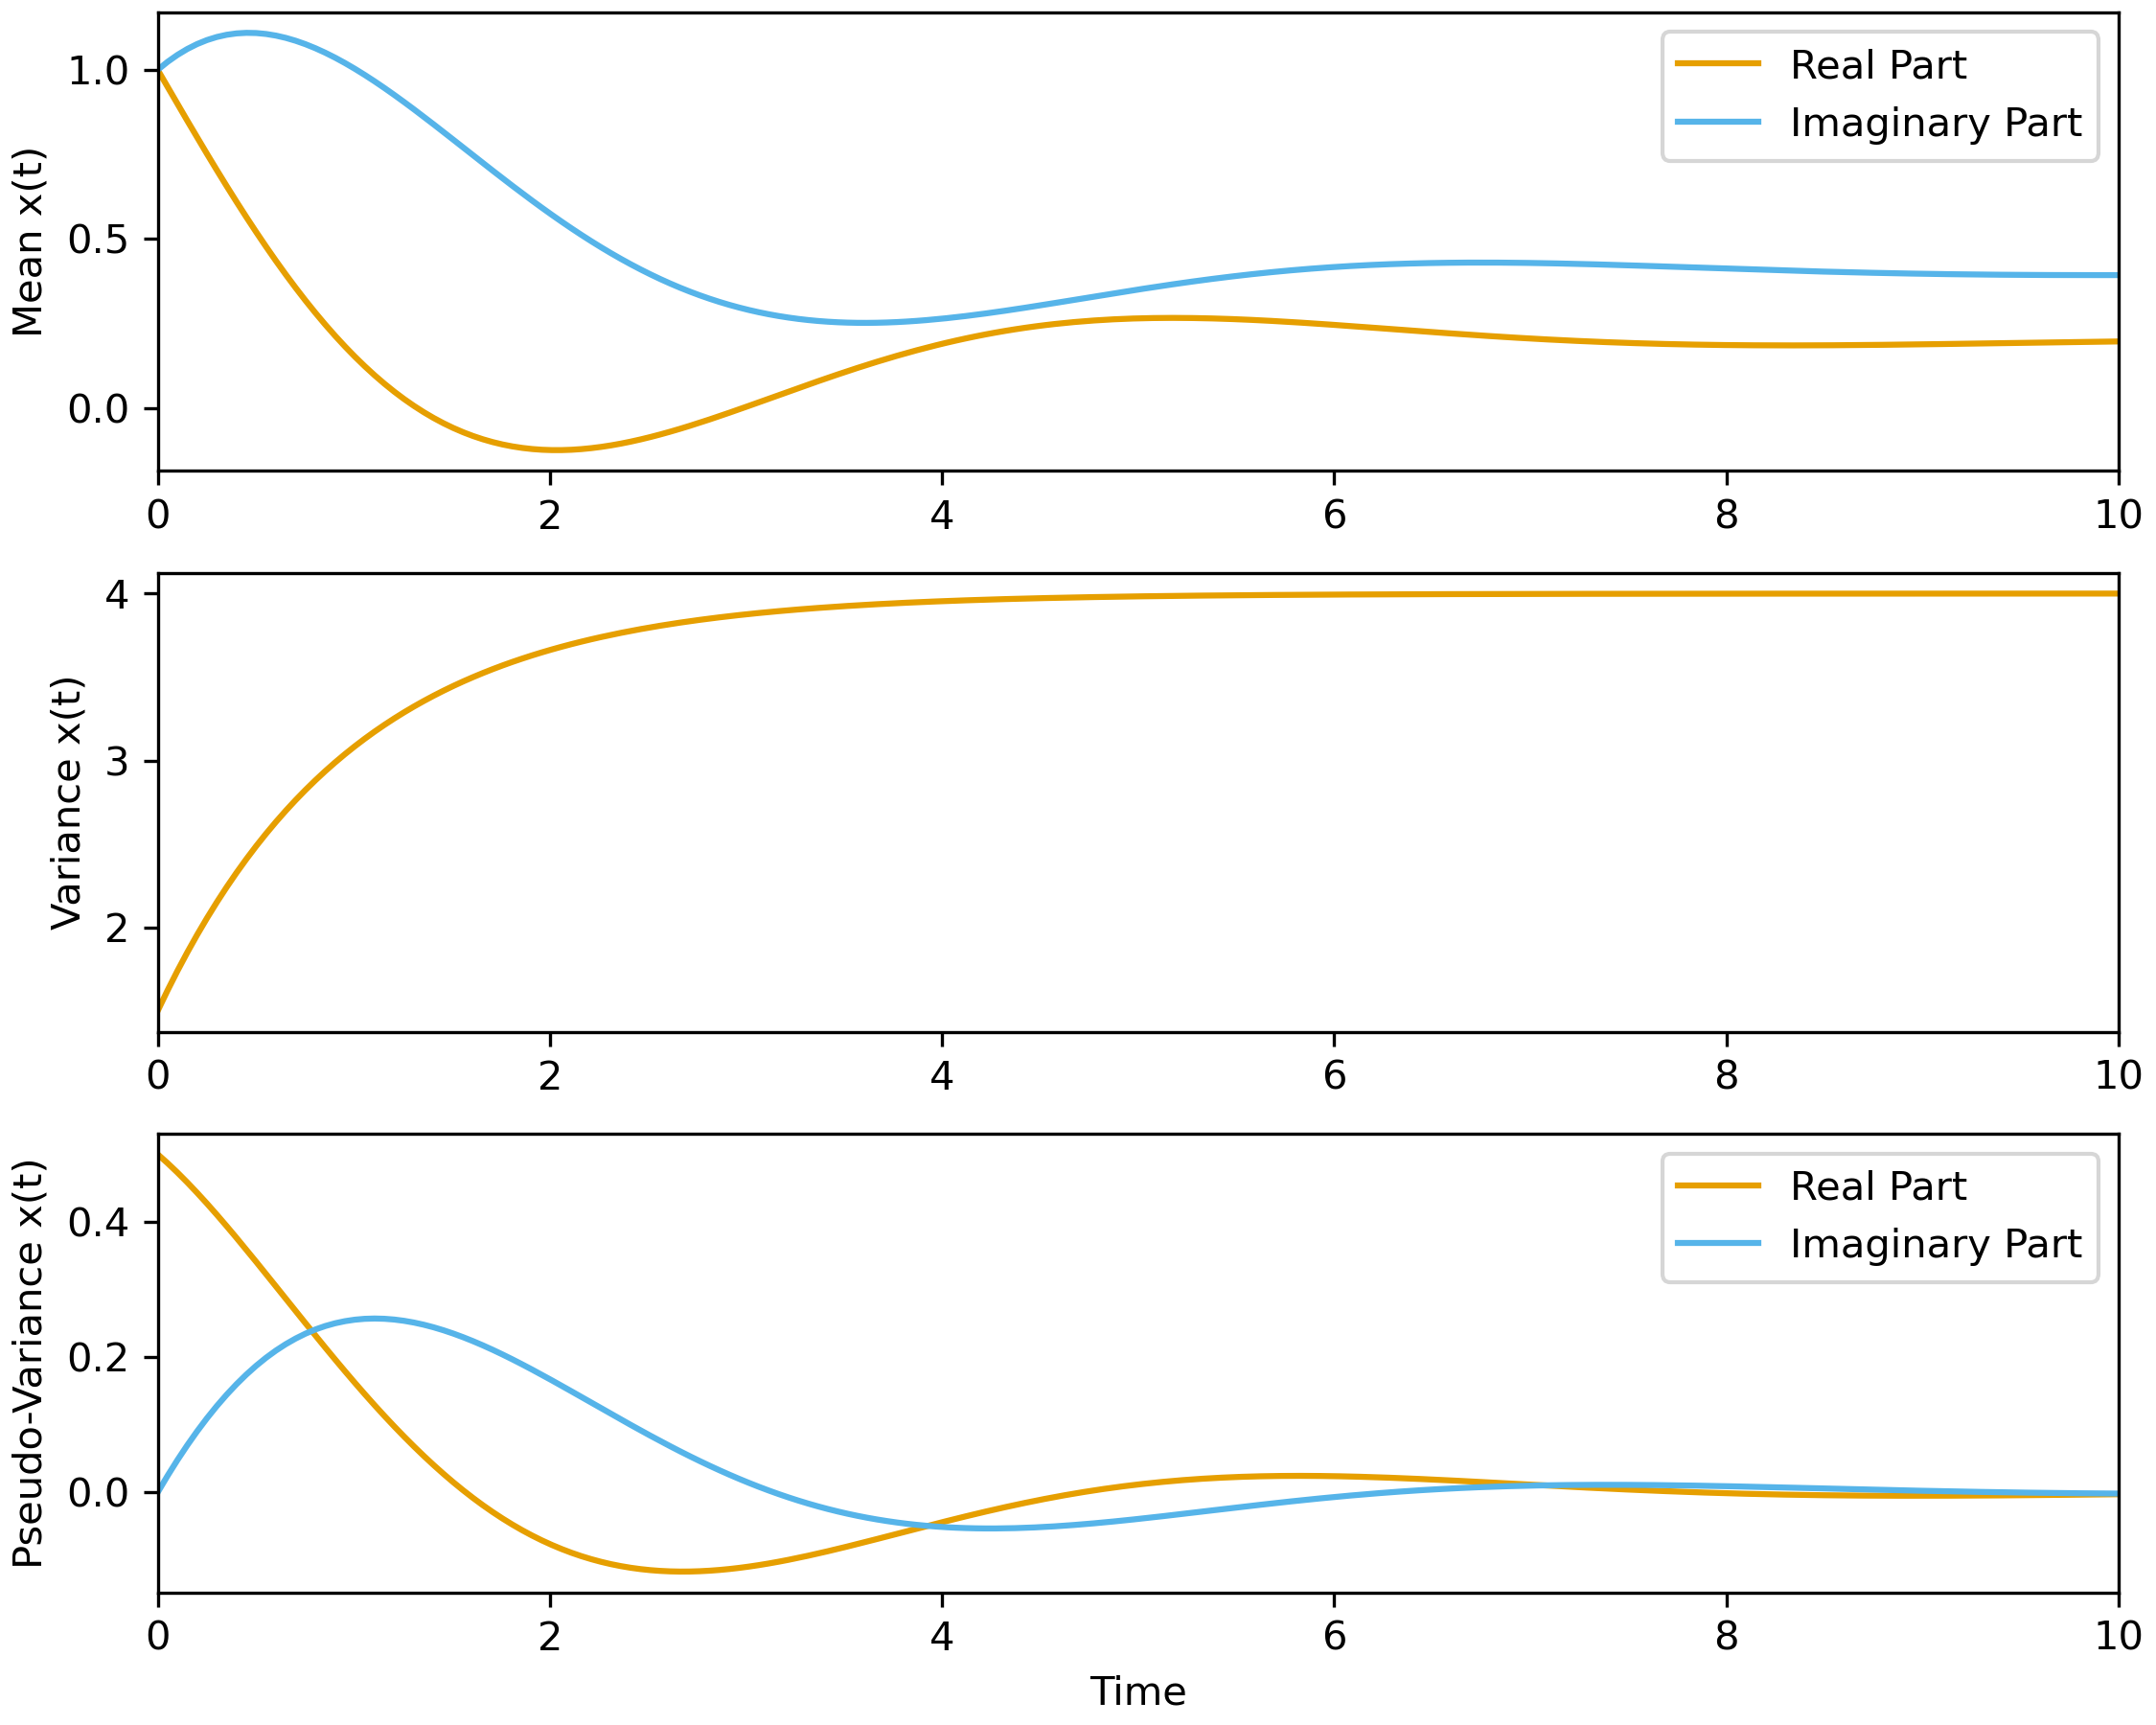
\includegraphics[width=0.75\textwidth]{../../src/3_stats.png}
	\caption{The mean (top), variance (center), and pseudo-variance (bottom) of the complex OU equations with $a = 0.5$, $\omega = 1.0$, $f = 0.5$, $\sigma = 2.0$, $\ev{\func{x}{0}} = 1 + i$, $\vr{\func{x}{0}} = 1.5$, and $\pvr{\func{x}{0}} = 0.5$.}
	\label{fig:stats_3}
\end{figure}
		
Source code is available from the GitHub repository
	
\begin{center}
	\url{https://github.com/jasonltorchinsky/MATH833_HW/releases/tag/hw2}
\end{center}

and is given in Appendix~\ref{app:code_3}. In short, the code takes a input parameters \texttt{-{}-decay} (or \texttt{-a}), \texttt{-{}-oscil} (or \texttt{-w}), \texttt{-{}-force} (or \texttt{-f}), and \texttt{-{}-stoch} (or \texttt{-s}) that correspond to $a$, $omega$, $f$ and $\sigma$, respectively. It then calculates the mean, variance, and covariance of $\func{x}{t}$ analytically using the previously derived formulas for $\ev{\func{x}{0}} = 1 + i$, $\vr{\func{x}{0}} = 1.5$, and $\pvr{\func{x}{0}} = 0.5$, and plots them.
